\documentclass[czech,master]{diploma}
\usepackage[autostyle=true,czech=quotes]{csquotes}
\usepackage[backend=biber, style=iso-numeric, alldates=iso]{biblatex}
\usepackage{dcolumn}
\usepackage{subfig}
\usepackage{hyperref}
\usepackage{xurl}
\usepackage{tikz}
\usepackage[cpp]{diplomalst}
\usepackage{amsfonts}
\usepackage{enumerate}

% \usepackage[dvipsnames]{xcolor}
\usepackage{listings}

\lstdefinelanguage{Kotlin}{
  comment=[l]{//},
  commentstyle={\color{gray}\ttfamily},
  emph={filter, first, firstOrNull, forEach, lazy, map, mapNotNull, println},
  % emphstyle={\color{OrangeRed}},
  % identifierstyle=\color{black},
  keywords={!in, !is, abstract, actual, annotation, as, as?, break, by, catch, class, companion, const, constructor, continue, crossinline, data, delegate, do, dynamic, else, enum, expect, external, false, field, file, final, finally, for, fun, get, if, import, in, infix, init, inline, inner, interface, internal, is, lateinit, noinline, null, object, open, operator, out, override, package, param, private, property, protected, public, receiveris, reified, return, return@, sealed, set, setparam, super, suspend, tailrec, this, throw, true, try, typealias, typeof, val, var, vararg, when, where, while},
  % keywordstyle={\color{NavyBlue}\bfseries},
  morecomment=[s]{/*}{*/},
  morestring=[b]",
  morestring=[s]{"""*}{*"""},
  ndkeywords={@Deprecated, @JvmField, @JvmName, @JvmOverloads, @JvmStatic, @JvmSynthetic, Array, Byte, Double, Float, Int, Integer, Iterable, Long, Runnable, Short, String, Any, Unit, Nothing},
  % ndkeywordstyle={\color{BurntOrange}\bfseries},
  sensitive=true,
  % stringstyle={\color{ForestGreen}\ttfamily},
}

\lstdefinelanguage{Tilscript}{
  comment=[l]{--},
  commentstyle={\color{gray}\ttfamily},
  morestring=[b]",
  keywords={Defn, Import, TypeDef, Struct},
  ndkeywords={Int, Real, Time, World, List, Tuple, If, Progn, MkTuple, Cond,
    ListOf, Bool, Construction, Any1, Any2, Any3, Any4, Any5, Any6, Any7, Any8,
    Any9},
  sensitive=true,
}

\lstset{language=Tilscript}

\newcommand{\peteref}[1]{\ref{#1}\,--\,\nameref{#1}}

\usetikzlibrary{fit}

\ThesisAuthor{Bc. Filip Peterek}
\ThesisSupervisor{prof. RNDr. Marie Duží, CSc.}
\CzechThesisTitle{Implementace jazyka TIL-Script}
\EnglishThesisTitle{Implementation of the TIL-Script Language}
\SubmissionYear{2023}

\ThesisAssignmentFileName{Figures/spec.pdf}
% TODO: Doplnit
% \Acknowledgement{Děkuji Adélce za to, že mě ignoruje, a já tak mám čas psát diplomovou práci.}

\CzechAbstract{
    Cílem práce je implementovat programovací jazyk TIL-Script. Jazyk TIL-Script slouží jako
    výpočetní varianta logického kalkulu TIL, jenž umožňuje jednoduchý strojový zápis konstrukcí
    Transparentní intenzionální logiky, ale také jejich následné provedení. Práce dále řeší
    praktické problémy s interpretací jazyka TIL-Script, a to například definice pojmenovaných
    funkcí, interakce s databází, apod. Dále se práce snaží navrhnout nadmnožinu jazyka TIL-Script,
    která umožní konstrukce TILu nejen provádět, ale také analyzovat, vytvářet je, a pracovat
    s nimi.
}

\CzechKeywords{
    Transparentní intenzionální logika, TIL-Script, překladač
}

\EnglishAbstract{
    The goal of the thesis is the definition and implementation of the TIL-Script language.
    TIL-Script is a scripting language which serves the purpose of a computational variant of
    Transparent intensional logic, a logical calculus based on typed lambda calculi. TIL-Script
    allows for not just representation, but also execution of TIL constructions. This work also
    deals with practical problems of TIL-Script implementation, such as definitions of named
    functions, interaction with databases, and so on. Furthermore, this thesis attempts to define
    a superset of the TIL-Script language, which allows for not just the execution of constructions,
    but also for their creation and analysis.
}

\EnglishKeywords{
    Transparent intensional logic, TIL-Script, interpreter
}

\AddAcronym{TIL}{Transparentní intenzionální logika}
\AddAcronym{JVM}{Java Virtual Machine}
\AddAcronym{JRE}{Java Runtime Environment}
\AddAcronym{JAR}{Java Archive}
\AddAcronym{TCO}{Tail Call Optimization}
\AddAcronym{REPL}{Read-Eval-Print Loop}
\AddAcronym{CLI}{Command Line Interface}
\AddAcronym{AST}{Abstract Syntax Tree}
\AddAcronym{GCC}{GNU Compiler Collection}
\AddAcronym{GNU}{GNU is not Unix}
\AddAcronym{RCE}{Remote Code Execution}

\addbibresource{Sources/biblatex-examples.bib}
\addbibresource{Sources/coffee.bib}

% Novy druh tabulkoveho sloupce, ve kterem jsou cisla zarovnana podle desetinne carky
\newcolumntype{d}[1]{D{,}{,}{#1}}

\renewcommand\lstlistingname{Ukázka}
% \renewcommand\listoflistingscaption{Seznam výpisů zdrojového kódu}
% \listoflistings

% Zacatek dokumentu
\begin{document}

% TODO: Uncomment
\MakeTitlePages

% TODO: Uncomment
% Jsou v praci obrazky? Pokud ano vysazime jejich seznam a odstrankujeme.
% Pokud ne smazeme nasledujici dve makra.
\listoffigures
\clearpage

% TODO: Uncomment
% Jsou v praci tabulky? Pokud ano vysazime jejich seznam a odstrankujeme.
% Pokud ne smazeme nasledujici dve makra.
\listoftables
\clearpage

% A nasleduje text zaverecne prace.
\chapter{Úvod}
\label{sec:Introduction}

% TODO: Ocitovat n-gramove modely, word2vec, ChatGPT
% GPT-3: https://arxiv.org/abs/2005.14165

Analýza přirozeného jazyka jako disciplína stále rychleji stoupá na oblibě i důležitosti. Jistě
málokomu unikly například n-gramové modely založené na predikci následujícího slova
z předcházejících $n$ slov, či vektorové modely jako Word2Vec, umožňující reprezentovat význam
slov pomocí vektorů. Poslední dobou se velmi často mluví o jazykovém modelu GPT-3.

Výčet přístupů k analýze přirozeného jazyka však nekončí n-gramy a neuronovými sítěmi.

\endinput

\chapter{Transparentní intenzionální logika}
\label{sec:TILIntroduction}

% TODO: Citace
Transparentní intenzionální logika (TIL) je logický systém založený na typovaném lambda kalkulu.
TIL je využíván k logické analýze přirozeného jazyka. Oproti tradičnímu lambda kalkulu, jenž
se využívá jako komputační model, tedy jako pouhý prostředek k dosažení konkrétní hodnoty --
výsledku, v Transparentní intenzionální logice hraje konstrukce kalkulu často důležitější roli,
než hodnota, kterou by konstrukce po provedení zkonstruovala.

Jako příklad využití lambda kalkulu jako výpočetní model lze uvést např. funkcionální programovací
jazyk Haskell. Interně je Haskell kompilován do lambda kalkulu (přesněji do jeho supersetu
obsahujícího např. čísla nebo logické hodnoty, která jinak v lambda kalkulu musíme kódovat pomocí
Churchova kódování -- K-kombinátorů, apod.). Ultimátně v Haskellu ovšem lambda kalkul slouží pouze
k získání konkrétního výsledku. Nadefinujeme vztah mezi vstupem a výstupem, a program napsaný
v Haskellu nám vstup transformuje. Pokud zanedbáme efektivitu programu, nezajímá nás, jakým
způsobem program spočítal výsledek, dokud jej spočítal správně.

Naopak Transparentní intenzionální logika je hyperintenzionálním kalkulem, který nám umožňuje
vytvářet konstrukce vypovídající o jiných konstrukcích. TIL vychází z myšlenky, že výraz
přirozeného jazyka sice označuje denotát -- konkrétní individuum, významem výrazu ovšem není
samotný denotát, který ani nemusí nutně existovat. Význam výrazu je abstraktní a lze jej zachytit
konstrukcí. Daná konstrukce poté při provedení zkonstruuje denotát výrazu. Jako příklad lze uvést
například výraz "francouzský král." V době psaní této práce Francie krále nemá. Výraz nemá žádný
denotát, neuvádí žádné konkrétní individuum. Přesto výrazu "francouzský král" rozumíme, výraz má
svůj význam, jen v současné době neuvádí žádnou osobu. A budeme-li chtít o významu výrazu
"francouzský král" něco vypovědět, například že francouzský král je monarchou v čele Francie,
daný monarcha nemusí existovat. Dále lze uvést například rozdíl mezi výrazy "logaritmus 1024
o základě 2" a "5 + 5". Denotátem obou výrazů je 10. Zadáme-li do interpreteru Haskellu výrazy
\lstset{language=Haskell}
\lstinline{logBase 2 1024} a \lstinline{5 + 5}, získáme v obou případech stejný výsledek.
V přirozeném jazyce ovšem chápeme značný rozdíl mezi oběma výrazy, ačkoliv mají stejný denotát.
"Logaritmus 1024 o základě 2" vyjadřuje číslo, kterým musíme umocnit dvojku, abychom získali 1024.
Výraz "5 + 5" očividně vyjadřuje úplně jinou matematickou operaci a jeho výsledek spočítáme jiným
postupem.

\begin{figure}
    \centering
    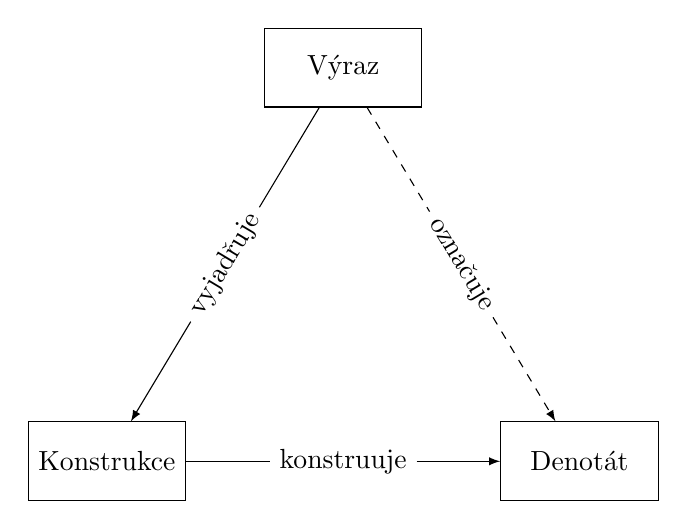
\begin{tikzpicture}
        \node[draw, fit={(0, 0) (2, 1)},              xshift=3cm, inner sep=0pt, label=center:Výraz] (A) {};
        \node[draw, fit={(0, 0) (2, 1)}, yshift=-5cm,             inner sep=0pt, label=center:Konstrukce] (B) {};
        \node[draw, fit={(0, 0) (2, 1)}, yshift=-5cm, xshift=6cm, inner sep=0pt, label=center:Denotát] (C) {};

        \path (A) -- node[sloped] (ab) {vyjadřuje}  (B);
        \path (A) -- node[sloped] (ac) {označuje}   (C);
        \path (B) -- node[sloped] (bc) {konstruuje} (C);

        \draw [-latex]          (A)--(ab)--(B);
        \draw [-latex] [dashed] (A)--(ac)--(C);
        \draw [-latex]          (B)--(bc)--(C);
    \end{tikzpicture}
    \caption{Schéma procedurální sémantiky TIL}
    \label{fig:til-semantics}
\end{figure}

Denotátem výrazu může být jak objekt z báze, konstrukce, i funkce.

Jak již bylo zmíněno, Transparentní intenzionální logika vychází z typovaného lambda kalkulu, proto
také každý objekt musí mít svůj typ. Pro správné pochopení TILu, a tedy i této práce, je tak nutné 
znát typovou hierarchii TIL.

\subsection{Báze}

Báze je kolekce vzájemně disjunktních neprázdných množin, které dohromady definují universum
diskurzu. Tyto množiny definují atomické objekty. Každá množina dále objektům určuje určitá
základní kritéria (např. pokud jako jednu z množin báze zvolíme množinu $\mathbb{N}$, víme, že
všechny objekty z této množiny budou čísla).

\subsection{Typy 1. řádu}


\subsection{Rozvětvěná hierarchie typů}

\subsection{Konstrukce TIL}

\subsection{Charakteristické rysy TIL}

\endinput

\chapter{TILScript}

Nyní konečně přišel čas představit TILScript. TILScript je interpretovaný funkcionální programovací
jazyk, do znatelné míry inspirovaný jazyky jako Haskell nebo Lisp. Syntax TILScriptu by měla co
nejvíce připomínat syntaktické prvky Transparentní intenzionální logiky, aby pouhá znalost TILu
stačila k okamžitému pochopení TILScriptu. Sémantika by poté měla být stejná.

Tato kapitola je rozdělena do tří sekcí. V první sekci jsou popsány důležité základní rysy
TILScriptu. Druhá sekce popisuje již existující prvky TILScriptu, a případně dokumentuje změny
oproti předchozím verzím TILScriptu. Poslední sekce se věnuje navrhovaným rozšířením jazyka
TILScript.

\section{Charakteristické rysy TILScriptu}

Tato sekce popisuje charakteristické rysy TILScriptu v takové podobě, jakou nabývá v této práci.
Pokud se v některém bodě TILScript neshoduje s TILem či předchozími verzemi TILScriptu, je rozdíl
náležitě popsán a vysvětlen.

\subsection{Lambda kalkul parciálních funkcí}

\subsubsection{Shora neomezená arita funkcí}

% TODO: Ozdrojovat currying asi? Idk, lambda kalkul

Narozdíl od lambda kalkulu ve své tradiční podobě, nebo například jazyka Haskell, v Transparentní
intezionální logice není arita funkce shora omezená. TILScript musí tento fakt reflektovat. Proto
tento jazyk umožňuje definici i aplikaci funkcí libovolné (samozřejmě nezáporné) arity. Také zde
neexistuje rozvíjení funkcí (anglicky \textit{currying}). Zatímco např. v Haskellu jsou funkce
arity dvě nebo vyšší automaticky rozvinuty na sérií několika unárních funkcí, jejichž oborem hodnot
jsou unární nebo nulární funkce, a jedné nulární funkce která vrací žádaný výsledek, v TILScriptu
není arita nijak omezená.

\subsubsection{Parciální funkce a respektování principu kompozicionality}

Jelikož v TIL můžou být funkce parciální, musí i TILScript počítat s parcialitou funkcí. Dále musí
TILScript respektovat princip kompozicionality, základní rys Transparentní intenzionální logiky.
Jedním z důsledků principu kompozicionality je, že konstrukce, jejíž přinejmenším jeden konstituent
je nevlastní, bude také nutně nevlastní. Reprezentaci stavu, kdy parciální funkce je aplikována
na argumenty, na kterých není definována, se věnuje podsekce \textit{Hodnota Nil} \ref{nil-value}
této kapitoly. Způsob dodržování principu kompozicionality je popsán v podsekci
\textit{Okamžité vyhodnocování (Eager evaluation)} \ref{eager-eval}.

%TODO: Ocitovat
Jedinou výjimkou je funkce \lstinline{IsNil}, jež vrací pravdivostní hodnotu \lstinline{True},
pokud je její jediný argument \lstinline{Nil}, v opačném případě je jejím výsledkem
\lstinline{False}. Tato speciální sémantika funkce \lstinline{IsNil}, ačkoliv porušuje princip
kompozicionality a vyžaduje aplikaci unární funkce na "nic," je zvolena jako doplněk k funkci
\lstinline{Improper/(o*_n)} definované v Průvodci čtenáře, a jako kompromis mezi dodržením
principů TIL a umožněním zpracování chyb.

\subsection{Neměnnost proměnných a symbolů (\textit{Immutability})}

Jelikož je TILScript funkcionální jazyk, jsou hodnoty všech proměnných konstantní -- tedy
jakmile je proměnné jednou přiřazena valuace, nelze její hodnotu změnit. Dále nelze proměnnou
zastínit (angl. \textit{to shadow, shadowing}) v rámci oblasti platnosti (angl. \textit{scope}),
ve které byla definována. Proměnnou lze zastínit vytvořením nové oblasti platnosti (tedy například
na novém rámci zásobníku, angl. \textit{stack frame}).

% TODO: symboly

\subsection{Okamžité vyhodnocování (\textit{Eager evaluation})} \label{eager-eval}

\subsection{}

\section{TILScript jako výpočetní varianta TILu}

\section{Rozšíření TILScriptu}

\subsection{Hodnota \textit{Nil}} \label{nil-value}

\endinput

\chapter{Implementace}

V této kapitole nastíníme implementační detaily interpreteru. Nejprve zmíníme využité technologie,
poté popíšeme architekturu projektu, nakonec pak uvedeme zajímavější problémy, které se objevily
při implementaci překladače, a jejich řešení.

\section{Zvolené technologie}

Celý projekt je implementován v jazyce \textbf{Kotlin} \footnote{Přestože je projekt psaný
  v Kotlinu, v práci často zmiňujeme např. \textit{Java knihovny}, \textit{Java objekty}, apod.
  Většinou tím myslíme Javu jako platformu. V takových případech poté nezáleží, zda
  používáme jazyk Java, Kotlin, nebo libovolný jiný jazyk kompilovaný pro platformu JVM.}.
Jazyk Kotlin je staticky typovaný, multiparadigmatický jazyk kompilovaný do \textbf{JVM} bytekódu.
Kotlin je vytvářen jako alternativa k jazyku Java, a nabízí plnou kompatibilitu s Javou. Využití
Kotlinu umožňuje využívat veškeré výhody Java ekosystému, včetně knihoven psaných v Javě, ale také
psát expresivnější kód, než by bylo možné v Javě. Null-safety a jazyková podpora pro algebraické
datové typy pak umožňují psát bezpečnešjí kód, než je možné v jazyce Java. Pro spuštění překladače
je samozřejmě nutné mít na počítači nainstalované JRE.

Jako build systém byl zvolen projekt \textbf{Gradle}. Důvodem této volby je relativní jednoduchost
konfigurace i využití systému Gradle, ale také přístup k Maven repozitáři s Java knihovnami. Dále
využíváme několik Gradle pluginů nutných k sestavení projektu.

Parser generujeme za pomoci technologie \textbf{Antlr} ve verzi 4. Antlr je open-source generátor
parserů podporující tvorbu parserů v řadě jazycích. V našem případě využíváme jako cílový jazyk
Javu.

Interpreter využívá knihovnu \lstinline{org.apache.commons:commons-text} pro zpracování escape
sekvencí. Tím výčet využitých technologií končí.

\section{Architektura projektu}

Celý projekt je rozdělen do čtyř komponent -- společné knihovny (\lstinline{common}), standardní
knihovny (\lstinline{stdlib}), překladače (\lstinline{interpreter}) a matematické knihovny
(\lstinline{math}). Schéma projektu je znázorněno v obrázku \ref{fig:project-structure}, který
vyjadřuje, jak na sobě jednotlivé komponenty projektu závisí.

\begin{figure}
    \centering
    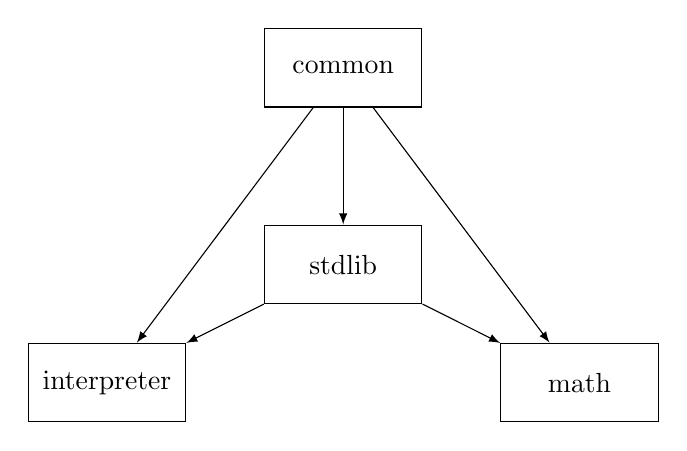
\begin{tikzpicture}
        \node[draw, fit={(0, 0) (2, 1)},                xshift=3cm, inner sep=0pt, label=center:common] (A) {};
        \node[draw, fit={(0, 0) (2, 1)}, yshift=-2.5cm, xshift=3cm, inner sep=0pt, label=center:stdlib] (B) {};

        \node[draw, fit={(0, 0) (2, 1)}, yshift=-4cm,   xshift=6cm, inner sep=0pt, label=center:math] (C) {};
        \node[draw, fit={(0, 0) (2, 1)}, yshift=-4cm,   xshift=0cm, inner sep=0pt, label=center:interpreter] (D) {};

        \draw [-latex]          (A)--(B);
        \draw [-latex]          (A)--(C);
        \draw [-latex]          (A)--(D);
        \draw [-latex]          (B)--(C);
        \draw [-latex]          (B)--(D);
    \end{tikzpicture}
    \caption{Komponenty projektu}
    \label{fig:project-structure}
\end{figure}

\subsection{Společná knihovna \lstinline{common}}

Knihovna \lstinline{common} obsahuje kód společný pro zbytek projektu. Jedná se například
o implementace tříd reprezentujících TIL konstrukce, definice společných rozhraní, reprezentaci
typů, nebo drobné utility. Knihovna neobsahuje definice TIL-Script objektů, slouží ke sdílení kódu
napříč jednotlivými komponentami. Využít ji tak může například programátor implementující novou
TIL-Script knihovnu, konečného uživatele se však existence \lstinline{common} nijak netýká.

Knihovna nemá žádné externí závislosti.

\subsection{Standardní knihovna \lstinline{stdlib}}

Knihovna \lstinline{stdlib} obsahuje implementaci standardní knihovny. \lstinline{stdlib}
nekonformuje vůči rozhraní, kterému musí konformovat TIL-Script knihovny implementované jako Java
knihovny a distribuované jako Java archivy. Standardní knihovnu překladač automaticky importuje
v každém souboru. Není tedy třeba ji importovat explicitně.

Standardní knihovna je nezávislá na použitém překladači TIL-Scriptu. Interpreter, jenž je součástí
projektu, můžeme klidně nahradit novým interpreter (za předpokladu, že daný interpreter implementuje
potřebná rozhraní, např. \lstinline{InterpreterInterface} definované v knihovně \lstinline{common}).
Interpreter samotný však na standardní knihovně závisí. Kvůli syntaktickému cukru
(funkce \lstinline{Cond}, \lstinline{ListOf}, atd.), funkci \lstinline{If}, jež musí být
vyhodnocována líně, apod., musí překladač obsahovat speciální podporu pro standardní knihovnu.

Standardní knihovna definuje základní množinu funkcí, hodnot, typů a proměnných potřebnou pro práci
s TIL-Scriptem.

\subsection{Matematická knihovna \lstinline{math}}

Matematická knihovna \lstinline{math} slouží jako ukázková implementace TIL-Script knihovny
v Kotlinu, případně v Javě. Dále je využívána k testování funkčnosti importování Java knihoven.
Narozdíl od standardní knihovny, překladač je naprosto nezávislý na knihovně \lstinline{math}.
\lstinline{math} je třeba importovat explicitně pomocí výrazu \lstinline{Import}.

Knihovnu nelze označit za extenzivní, obsahuje pouze malé množství funkcí, definice symbolických
hodnot \lstinline{E}, \lstinline{Pi} a proměnných \lstinline{e}, \lstinline{pi} aproximujících
eulerovo číslo a číslo $\pi$.

\subsection{Interpreter}

Narozdíl od předchozích komponent, které byly čistě Java knihovnami, Interpreter je spustitelný Java
program (tedy program s korektně definovanou funkcí \lstinline{main}). Jedná se o referenční
implementaci překladače jazyka TIL-Script. Překladač podporuje TIL-Script v takové podobě, v jaké je
definován touto prací. Obsahuje základní nástroje pro hlášení chyb, aby ulehčil práci
s TIL-Scriptem. Typovou kontrolu provádí pouze za běhu programu.

\section{Implementace překladače}

V této sekci nejprve nastíníme fungování překladače. Poté popíšeme zajímavé problémy týkající se
implementace překladače. Problémy můžou být zajímavé jak z hlediska řešeného problému, tak
z hlediska budoucího rozvoje.

\subsection{Vysokoúrovňový pohled na interpreter}

Interpreter funguje čistě jako neinteraktivní textová aplikace. Programy, které potřebujeme
interpretovat, předáváme překladači jako CLI argumenty. Pro překladač momentálně neexistuje žádné
grafické rozhraní, ani REPL, který by umožnil interaktivní překlad TIL-Script výrazů. Pokud
využíváme funkci \lstinline{main} definovanou v JAR překladače, spustí se programy sekvenčně
v takovém pořadí, v jakém je uživatel specifikoval. Pokud ale běh jednoho z programu skončí chybou,
další programy se již nespouští. Pro každý program je však vytvořena nová instance překladače. Běhy
jednotlivých programů jsou tedy na sobě nezávislé.

Pro strojovou práci se zdrojovým kódem musíme nejdříve daný kód převést ze sekvenční textové podoby
do reprezentace, se kterou počítač umí pracovat lépe. Proto programy převádíme do stromové
reprezentace nazývané abstraktní syntaktický strom (také AST -- Abstract Syntax Tree). Tomuto převodu
se říká \textit{parsování}, případně anglicky \textit{parsing}. Parsing (včetně tokenizace a
lexikální analýzy) je v našem interpreteru delegován parseru automaticky vygenerovaném technologií
Antlr. Pokud lexer nebo parser narazí na syntaktické chyby v programu, jsou dané chyby ohlášeny
uživateli a překlad automaticky končí neúspěchem. Výsledkem vygenerovaného parseru je abstraktní
syntaktický strom.

Výsledné AST je ovšem pro naše potřeby příliš generické. Antlr je nástroj pro všeobecné použití,
proto i pomocí Antleru vytvořené AST bývají všeobecné. Antlr však kromě parseru umí vygenerovat také
abstraktní třídu \lstinline{Visitor} sloužící k průchodu AST pomocí návrhového vzoru
\textit{visitor}. Pomocí visitoru převedeme výsledek parsování na dočasnou reprezantaci --
mezivýsledek. Tento výsledek je, díky omezením automaticky vygenerované třídy, stále nedostatečný.
V průběhu tohoto průchodu interpreter nehledá chyby v programu -- k tomu chybí překladači v současném
momentě dostatečný kontext.

Proto proces parsingu následuje ještě jeden průchod stromem a jeho konečný převod na přívětivou
strukturu. Během tohoto průchodu překladač převede reprezentaci zdrojového kódu na objekty tříd
definovaných v knihovně \lstinline{common} -- tedy na standardní objekty očekávané napříč projektem
(překladačem, funkcemi, apod.). Dále v tomto průchodu překladač provede expanzi funkcí
\lstinline{Cond}, \lstinline{ListOf}, \lstinline{TupleOf}, \lstinline{Progn} z variadických funkcí,
jež v TILu neexistují, na sekvenci binárních funkcí. Během tohoto průchodu může interpreter opět
zachytávat chyby -- většinou se jedná o chybné využití syntaktického cukru

Následně již dochází k interpretaci programu. Jednotlivé výrazy ovšem nejsou interpretovány přesně
v takovém pořadí, v jakém jsou v programu uvedeny. Při překladu jsou nejprve provedeny výrazy
\lstinline{Import}. Pokud překladač narazí na výraz \lstinline{Import}, je interpretace aktuálního
souboru pozastavena a překladač přeloží importovaný soubor. Po přeložení importované závislosti
jsou do kontextu současného souboru naimportovány symboly definované závislostí \footnote{
  Symboly zde myslíme názvy -- jména funkcí, proměnných, i symbolických hodnot. V daném kontextu
  slovo symbol nesouvisí se symbolickými hodnotami, využíváme jej stejně jako jej například
  využívají linkery kompilovaných programovacích jazyků.
}.

Dále dochází k přednostní deklaraci struktur, kterou následuje interpretace výrazů
\lstinline{TypeDef}. Teprve po interpretaci \lstinline{TypeDef} dojde ke korektní definic struktur
a jejich atributů. Využitím tohoto postupu umožníme, aby výrazy \lstinline{TypeDef} mohly zmiňovat
struktury, a aby v definicích struktur bylo možné zmiňovat typové aliasy.

Poté je potřeba provést deklarace proměnných a symbolických hodnot (viz \ref{symbolic-values}),
a současně deklarace a definice funkcí. V tomto kroku jsou deklarace proměnných automaticky
vyvozeny z definic. Pokud program obsahuje definici proměnné, není nutné dodávat deklaraci. Dodání
nekonfliktní deklarace ovšem není chybou.

Nakonec jsou interpretovány top-level konstrukce a přiřazení proměnným. Pokud je konstrukce
na nejvyšší úrovni $v$-nevlastní, program končí chybou. Pokud však uživatel počítá s tím, že
konstrukce může být $v$-nevlastní, může její výsledek přiřadit proměnné, nebo jej zpracovat
pomocí funkce \lstinline{IsNil}.

Vždy, když je vyhodnocována určitá skupina výrazů, ať už při přednostním vyhodnocování, nebo při
vyhodnocování konstrukcí, pořadí výrazů v konkrétní skupině vždy odpovídá jejich relativnímu pořadí
ve zdrojovém programu.

\subsection{Detaily implementace}

Tato podsekce popisuje detaily implementace, které můžou být důležité nebo zajímavé. Cílem je
vyzdvihnout řešení, které jsou důležité z hlediska budoucího rozvoje, řešení zajímavých problémů,
ale také řešení, které jsou suboptimální a zasloužily by si další vývoj.

\subsubsection{Interpretace konstrukcí a operace nad AST}

Velkým designovým rozhodnutím, a zároveň nedostatkem, je rozhodnutí operovat přímo nad abstraktním
syntaktickým stromem a interpretovat přímo TIL-Script konstrukce reprezentované Java objekty. Kód
není překládán do bytekódu, který by byl následně interpretován.

Tento přístup k interpretaci má velkou výhodu -- nízkou náročnost na implementaci. Překlad
do bytekódu by s sebou nesl značnou přidanou komplexitu. V první řadě by bylo potřeba implementovat
vlastní mechanismus zásobníku. V současné době TIL-Script sdílí zásobník s interpreterem. Aplikace
funkcí je řešena rekurzivně. Při aplikaci TIL-Script funkce volá interpreter interně vlastní metodu,
která aplikaci provede. S voláním metody na JVM je samozřejmě vytvořen nový rámec na zásobníku.
Na tomto rámci se poté uloží kontext aplikované TIL-Script funkce (argumenty funkce, apod.).
Po dokončení interpretace TIL-Script funkce se interpreter vrací z metody zpět na místo, odkud byla
metoda zavolána. S návratem je přirozeně spojena destrukce rámce na zásobníku -- destrukce, která
v současné implementaci obsahuje také zapomenutí kontextu funkce. Ten je poté uvolněn garbage
collectorem během reklamačního cyklu.

Právě garbage collector je druhou výhodou současného přístupu. Interpretace AST a využití mechanismu
zásobníku z JVM nám umožňuje využít také garbage collector z JVM pro automatickou správu paměti.
Pokud bychom implementovali vlastní zásobník nezávislý na JVM, museli bychom naprogramovat také
vlastní garbage collector.

Ve své podstatě však mechanismus stacku ani jednoduchý mark-and-sweep algoritmus\footnote{Myšleno
  mark-and-sweep algoritmus ve své nejjednodušší podobě. Mark-and-sweep algoritmus se používal již
  v padesátých letech minulého století, a používá se dodnes, v moderních jazycích je však silně
  optimalizován.} není složité naprogramovat.

Podstatně složitějším problémem by byla definice bytekódu, a také řešení oboustranného překladu mezi
bytekódem a JVM objekty.

% TODO: Continue

\subsubsection{Nezávislost knihoven na překladači}

Projekt je koncipován tak, aby byly TIL-Script knihovny nezávislé na intepreteru, který uživatel
použije. Implementovaný překladač je plně funkční, díky časovým omezením ovšem překladači chybí
některé nutné prvky, jako třeba optimalizace koncového volání (TCO), jež je ve funkcionálních
jazycích nezbytná, či překlad do bytekódu umožňující efektivnější překlad. V budoucnu se může stát,
že bude potřeba nahradit současný překladač efektivnější implementací. V takovém případě ovšem není
žádoucí, aby nastala potřeba přepsat nebo upravit také všechny již existující TIL-Script knihovny,
standardní knihovnu, apod. Pro implementaci TIL-Script knihovny je však potřeba, aby např.
TIL-Script funkce implementované v Javě měly určitý přístup k interpreteru, nebo alespoň kontextu,
ve kterém jsou volány. Jinak by tyto funkce nemohly přistupovat např. k proměnným, k jiným funkcím,
apod.

Za účelem odstranění závislosti na konkrétním překladači definuje knihovna \lstinline{common}
rozhraní \lstinline{InterpreterInterface}. Toto rozhraní specifikuje základní funkce, které
překladač TIL-Scriptu musí implementovat. Při volání TIL-Script funkcí definovaných pomocí Java
objektů je danému objektu předána instance překladače jako potomek \lstinline{InterpreterInterface}.

Tento princip je v softwarovém inženýrství velmi známý, je však nutné, aby na modularitu systému
bylo myšleno již od počátku a aby byl dobře zdokumentován. Tato práce umožňuje, aby bylo v budoucnu
možno vytvořit drop-in náhradu za konkrétní překladač bez jakékoliv úpravy existujícího kódu.

\endinput

\chapter{Uživatelská dokumentace}

Tato kapitola je věnována uživatelské dokumentaci. Součástí dokumentace je návod, jak spustit
TIL-Script program, popis standardní i matematické knihovny, návod na implementaci vlastní knihovny,
a nakonec také ukázka jednoduchého TIL-Script programu.

\section{Překlad programu}

\section{Standardní knihovna}

\section{Matematická knihovna}

\section{Implementace knihovny}

\section{Ukázka TIL-Script programu}

\endinput

\chapter{Závěr}

Cíl práce -- vytvořit funkční překladač jazyka TIL-Script, byl splněn. Byl implementován prototyp
překladače, který dokáže překládat programy jazyka TIL-Script, chybí mu ovšem některé v praxi
potřebné optimalizace (například optimalizace koncového volání). Nedostatky jsou však v textu
zdokumentovány, aby bylo možné překladač dále rozšiřovat a vylepšovat.

Dále práce rozšířila jazyk TIL-Script o nové prvky -- jako jsou například definice nových typů,
komentáře, výrazy \lstinline{Import}, nebo textové řetězce.

Implementována byla také standardní knihovna pro základní práci s jazykem TIL-Script, nebo
matematická knihovna definující několik užitečných matematických funkcí.

Překladač umožňuje implementovat TIL-Script funkce, které interně volají funkce jazyka Java -- tím
se jazyku TIL-Script otvírá také celý Java ekosystém, včetně knihoven pro jazyk Java.

Při tvorbě překladače bylo myšleno také na budoucí rozvoj. Současnou implementaci překladač je možné
nahradit implementací novou. Pokud bude nový překladač implementovat potřebná rozhraní, bude tento
překladač plně kompatibilní se standardní a matematickou knihovnou, případně s jakoukoliv jinou
knihovnou psanou pro jazyk TIL-Script.

\endinput


% Seznam literatury
\printbibliography[title={Literatura}, heading=bibintoc]

% Prilohy
\appendix
\chapter{Ukázky zdrojových kódů}

\lstinputlisting[caption={Ukázka definice intenzí.}]{SourceCodes/Intensions.tils}

\clearpage

\lstinputlisting[caption={Ukázka implementace registrátoru v jazyce Kotlin},language=Kotlin]{SourceCodes/Registrar.kt}

\clearpage

\lstinputlisting[caption={Ukázka implementace TIL-Script funkce v jazyce Kotlin},language=Kotlin]{SourceCodes/Function.kt}

\clearpage

\endinput


\end{document}
